\documentclass{IEEEtran}
\usepackage{cite}
\usepackage{amsmath,amssymb,amsfonts}
\usepackage{algorithmic}
\usepackage{graphicx}
\usepackage{textcomp}
\def\BibTeX{{\rm B\kern-.05em{\sc i\kern-.025em b}\kern-.08em
    T\kern-.1667em\lower.7ex\hbox{E}\kern-.125emX}}
\begin{document}
\title{A Priority-Aware Blockchain-Backed Secure Healthcare Record System Using AES-GCM and Threshold Secret Sharing}
\author{\IEEEauthorblockN{\textbf{Author 1}, \textbf{Author 2}, \textbf{Author 3}}
\IEEEauthorblockA{Indian Institute of Information Technology Kottayam, India\\
Guide: Dr. Lavanya Settupally\\
Email: author1@iiitkottayam.ac.in, author2@iiitkottayam.ac.in, author3@iiitkottayam.ac.in}}

\maketitle

\begin{abstract}
Healthcare data exchange across institutions requires strong confidentiality, integrity, and auditability while supporting timely access during critical medical events. This paper presents a hybrid, priority-aware secure healthcare record system that stores encrypted patient documents off-chain and commits immutable metadata and audit logs to a permissioned blockchain (Hyperledger Fabric). A Trusted Authority service performs document triage using an LLM to classify medical priority (HIGH/MEDIUM/LOW), then encrypts records using Advanced Encryption Standard--Galois/Counter Mode (AES-GCM) with contextual binding through Additional Authenticated Data (AAD). To avoid single-key compromise, the per-record encryption key is split using Shamir secret sharing and wrapped under per-peer Node Master Keys (NMKs) before being recorded on-chain. The system supports condition-wise record keys (e.g., patient\_id\_condition) to isolate unrelated medical conditions and enforces monotonic priority per record to prevent security downgrade on updates. A Streamlit dashboard enables hospital uploads and doctor reconstruction with role-based JWT authentication, while a Node.js Fabric gateway bridges the Trusted Authority to the blockchain network. The prototype demonstrates end-to-end workflows for upload, reconstruction, update, and version history retrieval, and provides a foundation for future quantitative benchmarking and multi-organization deployment.
\end{abstract}

\begin{IEEEkeywords}
AES-GCM, blockchain, healthcare data security, Hyperledger Fabric, secret sharing, trusted authority
\end{IEEEkeywords}

\section{Introduction}
\label{sec:introduction}
Secure sharing of healthcare records is a long-standing challenge because patient documents are sensitive, large, and frequently updated across multiple stakeholders such as hospitals, clinicians, and laboratories. Centralized storage solutions simplify deployment but introduce a single point of failure and often provide limited, non-tamper-evident auditability. Public blockchains provide immutability but are typically unsuitable for medical records due to privacy requirements, governance constraints, and the inefficiency of storing large payloads on-chain.

Permissioned blockchains such as Hyperledger Fabric enable controlled membership and immutable logging, yet naive approaches that store raw medical content on the ledger can still leak sensitive information and incur unnecessary storage costs. In parallel, clinical triage systems increasingly use machine learning to prioritize cases based on severity, but the priority output is rarely integrated into the security policy of data sharing.

This work addresses these gaps by proposing a hybrid architecture in which only cryptographic metadata and audit trails are stored on-chain, while patient documents remain encrypted off-chain. A Trusted Authority service performs priority classification using an LLM, encrypts records using AES-GCM with Additional Authenticated Data (AAD) binding, and applies threshold secret sharing to reduce the impact of key compromise. The system also supports condition-wise record identifiers and enforces monotonic priority per record key to prevent policy downgrade during updates. The remainder of this paper details the related work, methodology, implementation, experimental setup, results, and advantages of the proposed approach.

\subsection{Threat Model and Design Goals}
We assume an adversary may attempt to (i) access medical records without authorization, (ii) tamper with record history, or (iii) exfiltrate encryption keys from a subset of infrastructure nodes. The primary goals are confidentiality of medical content, integrity of stored ciphertext and metadata, auditable access, and controlled key reconstruction without trusting any single storage or compute node.

\subsection{Contributions}
The main contributions of this work are as follows: (i) a hybrid blockchain-backed architecture that stores only minimal metadata on-chain and encrypted medical content off-chain; (ii) a priority-aware access policy where an LLM-derived priority determines the threshold for secret reconstruction; (iii) an NMK-wrapped threshold key management approach that reduces the blast radius of compromise; and (iv) condition-wise identifiers with monotonic priority to prevent downgrade and cross-condition coupling during updates.

\section{Related Work / Literature Review}
Prior research explores blockchain-enabled healthcare data management for integrity, access logging, and cross-institution sharing. Azaria \emph{et al.} introduced MedRec, demonstrating blockchain-driven audit and permission management but relying on external storage and complex access workflows \cite{b1}. Xia \emph{et al.} proposed a data-sharing model that combines blockchain indexing with off-chain storage, yet requires careful key management and policy enforcement \cite{b2}. A survey by Hasselgren \emph{et al.} highlights that while blockchain improves provenance, medical privacy and scalability remain open problems, motivating hybrid designs \cite{b3}.

Hyperledger Fabric has been adopted in multiple healthcare prototypes due to its permissioned governance and modular endorsement policies \cite{b4}. However, many Fabric-based approaches still assume centralized encryption key custody, which becomes a single point of compromise. Cryptographic solutions for distributed access control include authenticated encryption (e.g., AES-GCM) and threshold secret sharing. NIST standardizes AES-GCM as an authenticated encryption mode suitable for protecting both confidentiality and integrity \cite{b5}. Shamir's secret sharing scheme provides information-theoretic guarantees for key splitting, supporting threshold reconstruction \cite{b6}.

Recent work also explores ML-assisted triage for prioritizing medical events. While learning-based triage improves clinical responsiveness, it is typically not coupled with cryptographic access control. Our work improves prior systems by (i) integrating LLM-driven priority into the security policy via threshold selection, (ii) preventing single-key compromise through Shamir sharing and NMK wrapping, (iii) storing only metadata and immutable audit logs on Fabric, and (iv) supporting condition-wise record keys and monotonic priority to avoid cross-condition interference and downgrade.

Additional studies propose privacy-preserving healthcare record sharing using off-chain encrypted storage anchored by on-chain indices \cite{b11}. Hardjono \emph{et al.} discuss interoperability requirements for blockchain-enabled health systems, emphasizing governance and cross-network identity management \cite{b12}. Androulaki \emph{et al.} detail Fabric's modular consensus and endorsement model, enabling access control policies beyond public blockchain capabilities \cite{b7}. Beyond healthcare, hybrid blockchain designs commonly separate data-plane storage from control-plane provenance to reduce cost and improve confidentiality \cite{b9}. These results motivate the proposed design, which aligns clinical priority with cryptographic policy and provides tamper-evident auditing without exposing medical content.

\subsection{Summary of Gaps Addressed}
Based on the above literature, the key limitations addressed by this project are: (i) insufficient separation between medical payload storage and immutable audit trails, (ii) single-point key custody in many hybrid blockchain designs, and (iii) lack of integration between clinical priority (triage) and the cryptographic access policy. The proposed design directly implements these missing elements using threshold secret sharing with NMK wrapping, Fabric-based audit logs, and an LLM-driven priority-to-threshold policy.

\subsection{Comparative Analysis with Existing Approaches}
Table~\ref{tab:comp} compares representative approaches discussed in the literature review with the proposed system. The comparison highlights that prior systems often provide auditability through blockchain, but do not couple clinical priority to cryptographic enforcement or distribute key custody using threshold secret sharing.

\begin{table}[!t]
\caption{Comparative Analysis with Existing Approaches}
\label{tab:comp}
\centering
\footnotesize
\setlength{\tabcolsep}{3pt}
\resizebox{\columnwidth}{!}{%
\begin{tabular}{|p{72pt}|p{62pt}|p{62pt}|p{62pt}|p{70pt}|}
\hline
\textbf{Approach} & \textbf{Encryption / Storage} & \textbf{Access Control} & \textbf{Blockchain Usage} & \textbf{Key Management / Priority} \\
\hline
MedRec \cite{b1} & Off-chain data pointers & Permissions via policy rules & Audit and access logs & No threshold sharing; no priority-aware enforcement \\
BBDS \cite{b2} & Cloud/off-chain storage & Access via sharing policies & Indexing/provenance & Centralized or single-custodian keys; no priority mapping \\
Hybrid off-chain storage \cite{b11} & Off-chain encrypted payloads & Policy-based access & On-chain references & Encryption without threshold key splitting; no priority-aware thresholds \\
\textbf{This project} & Off-chain AES-GCM ciphertext & JWT roles + threshold reconstruction & Metadata + wrapped shares + audit logs & Shamir $k$-of-$n$ with NMK wrapping; priority-to-threshold mapping \\
\hline
\end{tabular}%
}
\end{table}

\section{Proposed System / Methodology}
\subsection{System Architecture}
The proposed system consists of (i) a Trusted Authority (TA) service implemented using FastAPI, (ii) a permissioned Hyperledger Fabric network that stores record metadata and audit logs, (iii) an off-chain encrypted object store for patient documents, (iv) an LLM-based triage module for priority classification, and (v) a Node.js Fabric gateway that bridges the TA to Fabric. The TA provides role-based APIs for hospitals (upload) and doctors (read/update) using JSON Web Tokens (JWTs).

\begin{figure}[!t]
\centering
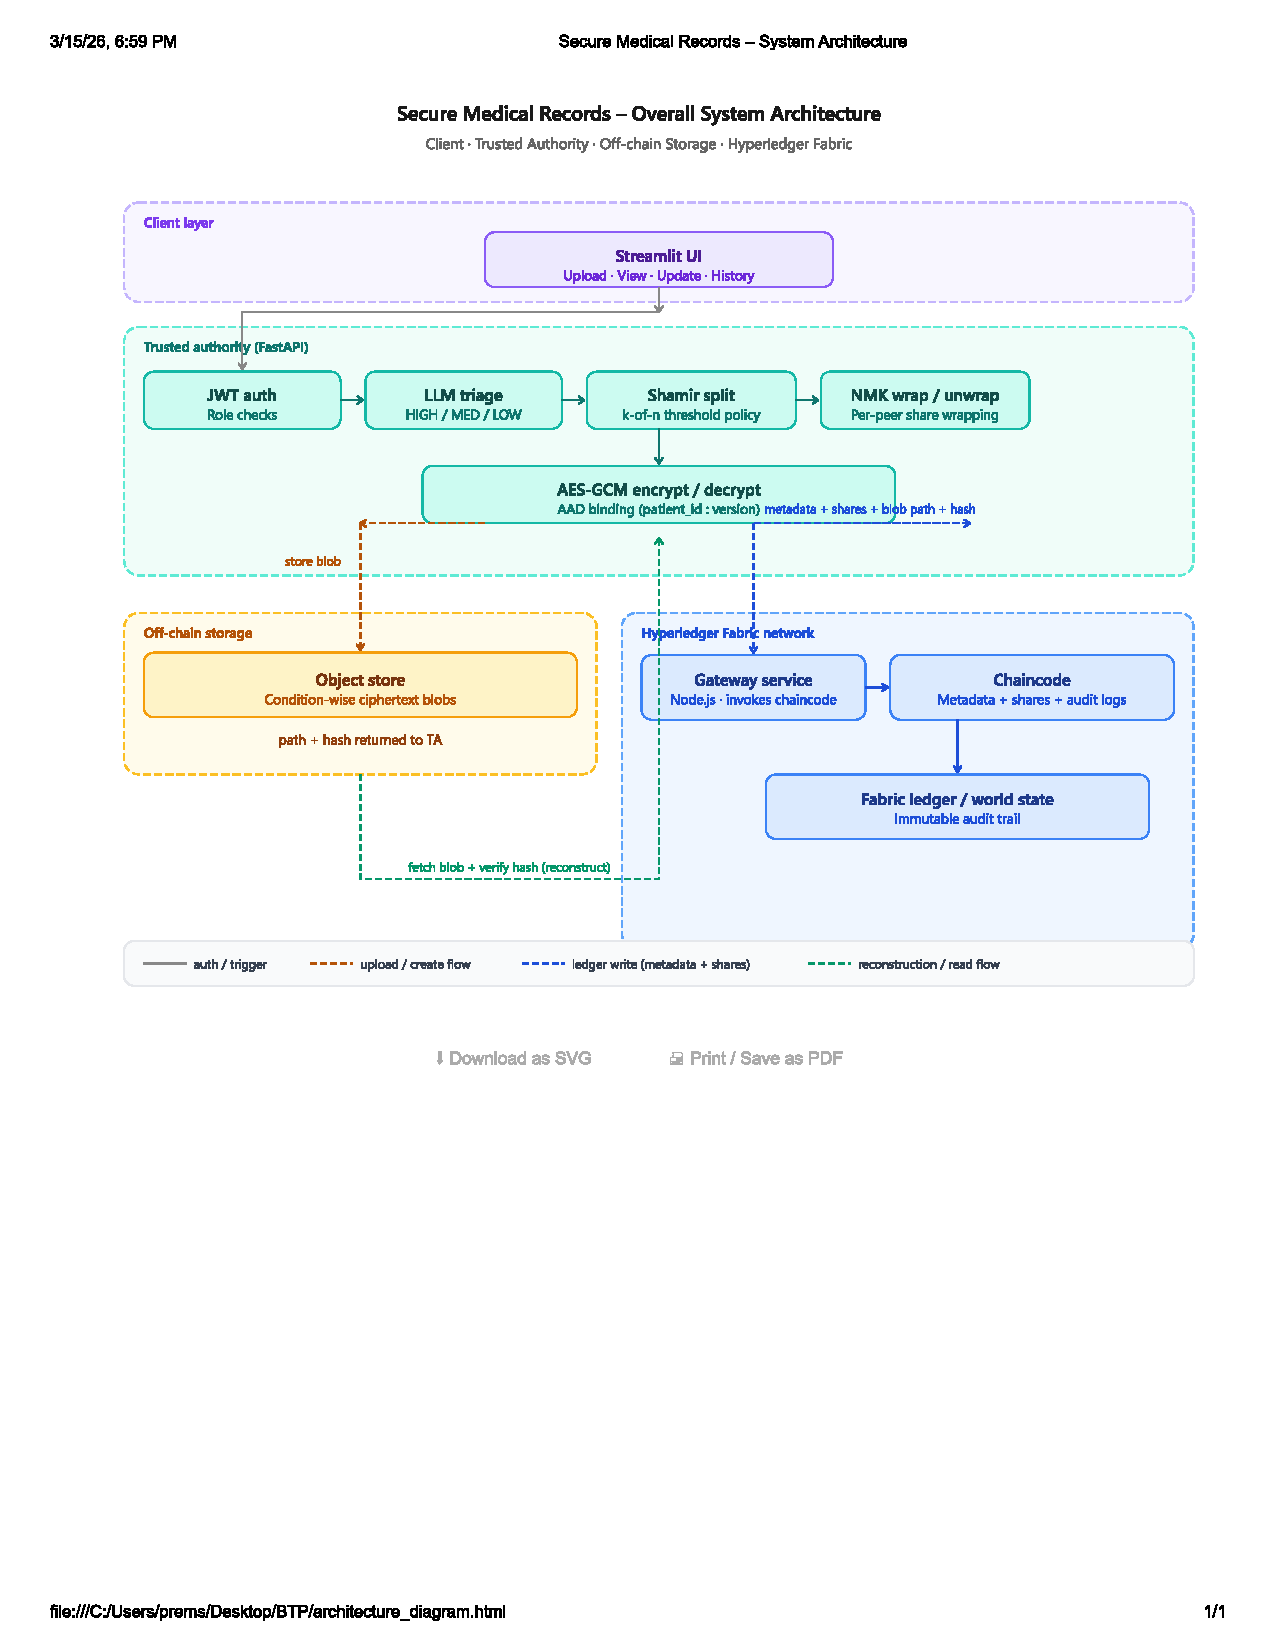
\includegraphics[width=\columnwidth]{arch.png}
\caption{System architecture of the proposed healthcare record platform showing the Streamlit UI, Trusted Authority (FastAPI) with triage and cryptographic modules, off-chain encrypted storage, and Fabric ledger accessed via a gateway for metadata and audit logging.}
\label{fig1}
\end{figure}

\subsection{System Modules}
The overall system is partitioned into four modules with clear trust boundaries. \textbf{(i) User interface module:} a Streamlit dashboard used by hospitals and doctors for authentication and record operations. \textbf{(ii) Trusted Authority module:} the core security service that performs triage, encryption, key splitting, and reconstruction. \textbf{(iii) Storage module:} an off-chain object store that persists encrypted blobs and exposes only file paths and hashes to other modules. \textbf{(iv) Blockchain module:} Hyperledger Fabric chaincode responsible for storing metadata, versions, and audit logs.

\subsection{Workflow}
For a new upload, the TA first classifies the record using the triage module and maps the resulting priority to a reconstruction threshold $k$. It then generates a per-record data key, encrypts the document using AES-GCM, and binds the ciphertext to the context using Additional Authenticated Data (AAD) set to \texttt{patient\_id:version}. The data key is split into $n$ Shamir shares with threshold $k$, and each share is wrapped under a peer-specific Node Master Key (NMK) before being stored as metadata on-chain. The encrypted document is stored off-chain with a content hash recorded on-chain for integrity checking.

For reconstruction, an authorized doctor requests the latest record. The TA retrieves the latest on-chain metadata, unwraps at least $k$ shares, reconstructs the data key, verifies the encrypted blob hash, and decrypts the ciphertext using the same AAD context.

\subsection{Priority Policy and Threshold Selection}
The project uses a simple, configurable mapping from priority to threshold. The objective is to increase compromise resistance for high-priority records while still allowing reconstruction when some peers are unavailable. In the current codebase, the mapping is implemented as a policy function (e.g., LOW$\rightarrow2$, MEDIUM$\rightarrow3$, HIGH$\rightarrow4$ for $n=5$ peers). The TA enforces \emph{monotonic priority}: if an update is later classified with a lower priority than the existing record, the system retains the higher priority and the corresponding threshold.

\subsection{Record Identity and Condition-wise Isolation}
Records are identified using a patient-condition key (e.g., \texttt{15\_HA}). This provides isolation between conditions and prevents unrelated updates from changing each other’s version history. Off-chain storage follows the same isolation principle by storing ciphertext in condition-wise folders, allowing independent lifecycle management.

\subsection{Core Algorithm}
The algorithm integrates triage-driven policy with authenticated encryption and threshold key management. The priority output $p\in\{\mathrm{LOW},\mathrm{MEDIUM},\mathrm{HIGH}\}$ is mapped to a threshold $k$ using a fixed policy. The TA enforces monotonic priority by comparing the newly predicted priority with the existing on-chain priority for the same patient-condition key.

\begin{algorithmic}
\STATE \textbf{Input:} patient\_key, file\_bytes, filename, requester
\STATE latest $\leftarrow$ getLatestRecord(patient\_key) (if exists)
\STATE version $\leftarrow$ 1 if latest is null else latest.version + 1
\STATE $p_{llm} \leftarrow$ LLM\_Triage(file\_bytes, filename)
\STATE priority $\leftarrow$ maxPriority(latest.priority, $p_{llm}$)
\STATE $k \leftarrow$ PriorityToThreshold(priority)
\STATE aad $\leftarrow$ Encode(patient\_key || ':' || version)
\STATE pdk $\leftarrow$ Random(32)
\STATE (nonce, ciphertext) $\leftarrow$ AESGCM\_Encrypt(pdk, file\_bytes, aad)
\STATE blob $\leftarrow$ nonce || ciphertext
\STATE (path, hash) $\leftarrow$ ObjectStore\_Put(patient\_key, version, blob)
\STATE shares $\leftarrow$ ShamirSplit(pdk, n, k)
\STATE wrapped\_shares $\leftarrow$ WrapWithNMK(shares, aad)
\STATE rec $\leftarrow$ \{patient\_key, priority, k, version, path, hash, wrapped\_shares, audit\_log\}
\STATE if version == 1 then ChaincodeCreate(rec) else ChaincodeUpdate(rec)
\STATE \textbf{Output:} \{patient\_key, priority, k, version\}
\end{algorithmic}

\subsection{Reconstruction Procedure}
Reconstruction is initiated by an authorized doctor. The TA queries Fabric for the latest record metadata, verifies role permissions, and collects at least $k$ wrapped shares. Each share is unwrapped using the corresponding NMK and the same AAD binding. The TA reconstructs the per-record data key using Shamir reconstruction, retrieves the encrypted blob from off-chain storage, verifies the stored hash, and then decrypts using AES-GCM. A successful read appends an immutable READ audit entry.

\subsection{Condition-wise Keys and Monotonic Priority}
To support multiple medical conditions per patient without interference, record identifiers follow the pattern \texttt{patient\_id\_condition} (e.g., \texttt{15\_HA}). Each identifier maintains independent version history. To prevent security downgrade, the system enforces monotonic priority per identifier: once a record key reaches a higher priority, subsequent updates cannot reduce it.



\subsection{Data Model Committed to the Ledger}
For each patient-condition key, the blockchain stores a compact record containing: current priority and threshold, version number, encrypted blob path, ciphertext hash (SHA-256), wrapped key shares indexed by peer identifiers, timestamps, and an append-only audit log recording CREATE/UPDATE/READ events. This design maintains ledger scalability by avoiding raw medical payloads on-chain.

\subsection{On-chain Versioning and Audit Trails}
Each record update creates a new immutable version entry rather than overwriting the previous one. Chaincode supports retrieving the latest version pointer and full history for a given patient-condition key. Audit logs are appended on every CREATE/UPDATE/READ operation and are stored alongside metadata, enabling traceability for compliance and incident response.

\section{Experimental Setup}
The experimental evaluation is designed to measure the overhead and behavior introduced by combining off-chain encrypted storage with on-chain metadata commits and threshold-based key reconstruction. The setup focuses on end-to-end workflows implemented in the project: upload (triage + encryption + secret sharing + ledger commit), reconstruction (ledger read + share unwrap + key reconstruction + decryption), update (versioning), and history/audit retrieval.

\subsection{Testbed and Deployment Topology}
Experiments are conducted on a local workstation environment (Windows with WSL2) where the system components run as separate processes/services: (i) the Trusted Authority (TA) FastAPI server, (ii) the Streamlit UI dashboard, (iii) the Node.js Fabric gateway REST service, (iv) a Hyperledger Fabric network and chaincode, and (v) a local off-chain object store used to persist encrypted blobs. The TA communicates with the gateway over HTTP(S), and the gateway submits/evaluates transactions against Fabric.

\subsection{Fabric Network Configuration}
The Fabric network is configured as a permissioned deployment suitable for prototyping. Chaincode implements record create/update, latest-read, history query, and audit append. The ledger stores only metadata and NMK-wrapped shares, while ciphertext is stored off-chain. For controlled experiments and offline validation, the TA can alternatively switch to a mock Fabric adapter that preserves the same record semantics.

\subsection{Workloads and Input Documents}
Workloads consist of representative healthcare documents (text/PDF) of varying sizes to study scaling of encryption and storage overhead. Each workload run issues a sequence of operations over one or more patient-condition keys: initial create, one or more updates, repeated reconstructions, and history retrieval. Condition-wise identifiers (e.g., \texttt{patient\_id\_condition}) are included to validate isolation across conditions.

\subsection{Cryptographic and Policy Parameters}
The TA generates a fresh per-record data key per version, encrypts using AES-GCM, and binds ciphertext to context using AAD set to \texttt{patient\_id:version}. The data key is split into $n$ Shamir shares with threshold $k$, where $k$ is selected by a priority-to-threshold policy based on triage output. To analyze the security--availability trade-off, experiments vary $k$ (while keeping $n$ fixed) and verify that reconstruction succeeds only when at least $k$ shares are available.

\subsection{Measurement Methodology}
We measure end-to-end latency for each workflow stage by instrumenting the TA at key boundaries: triage call, AES-GCM encryption/decryption, Shamir split/reconstruction, NMK wrap/unwrap, object store put/get, and Fabric transaction submission/evaluation. Measurements are repeated across multiple runs to reduce noise; results are summarized using distributional statistics (e.g., median and tail percentiles) rather than single-point values. In addition to latency, we report qualitative storage overhead by separating payload bytes stored off-chain from metadata stored on-chain.

\subsection{Functional and Security Validation}
Beyond performance methodology, the evaluation includes negative tests that validate security properties: (i) unauthorized requests without valid JWTs are rejected, (ii) tampering with off-chain ciphertext triggers hash verification failure, and (iii) replay attempts with mismatched AAD fail AES-GCM authentication. These checks ensure that measured behavior corresponds to the intended threat model.

\section{Implementation Details}
\label{sec:implementation}

\subsection{Technology Stack}
The Trusted Authority is implemented in Python using FastAPI and Pydantic for API validation. The Streamlit dashboard provides a lightweight web interface for hospital and doctor roles. A Node.js REST gateway uses the Hyperledger Fabric Gateway SDK to submit and evaluate chaincode transactions. The Fabric network uses chaincode written in JavaScript to store and retrieve metadata.

\subsection{Core Modules}
\textbf{Trusted Authority Core:} Implements upload, update, reconstruction, and history retrieval. It orchestrates LLM triage, AES-GCM encryption/decryption, Shamir split/reconstruction, and NMK wrapping.

\textbf{Object Store:} Stores encrypted blobs off-chain in a condition-wise directory structure and returns a SHA-256 hash for integrity.

\textbf{Fabric Adapter and Gateway:} The TA communicates with Fabric either through a mock ledger for development or via the Node.js gateway REST interface. A configurable SSL verification option supports development environments with self-signed certificates.

\subsection{Cryptographic Details}
AES-GCM provides authenticated encryption by producing a ciphertext and an authentication tag bound to both the plaintext and the Additional Authenticated Data. The project sets AAD to the patient identifier and version, ensuring that ciphertext cannot be replayed under a different context. Shamir secret sharing splits the per-record data key into $n$ shares, requiring any $k$ shares for reconstruction. NMK wrapping encrypts each share under a peer-specific master key before committing shares on-chain, so that leakage of ledger state alone does not reveal usable secret shares.

\subsection{Security Analysis}
This subsection summarizes how the project’s design choices mitigate practical threats in a permissioned healthcare setting.

\subsubsection{Adversary Model}
We consider adversaries who may (i) obtain read access to the ledger state, (ii) compromise a subset of logical peers and exfiltrate their NMKs, (iii) tamper with off-chain ciphertext blobs, (iv) attempt replay of ciphertext across patients or versions, or (v) abuse application credentials to access records outside their role.

\subsubsection{Attack Scenarios and Mitigations}
\textbf{Ledger disclosure:} Fabric stores only metadata and NMK-wrapped shares; plaintext never appears on-chain. Disclosure of ledger state alone is insufficient to recover the record key. \textbf{Single peer compromise:} a single NMK reveals at most one share; reconstruction requires at least $k$ shares. \textbf{Off-chain tampering:} the ciphertext hash stored in metadata is verified at reconstruction time; mismatches are detected. \textbf{Replay across records:} AAD binding ties encryption to \texttt{patient\_id:version}; decryption fails if the context differs. \textbf{Privilege misuse:} JWT role checks restrict endpoints, and all actions append immutable audit events.

\subsubsection{Residual Risks}
As a prototype, the system assumes secure handling of JWT secrets and NMKs on the host machine. In production, these should be stored in a secrets manager and protected by hardware-backed key storage where available.

\subsection{Chaincode Functions}
The Fabric chaincode implements record create, update, latest-read, history query, and audit append. Records are stored under composite keys \texttt{record(patientId, version)} while a \texttt{latest(patientId)} pointer tracks the most recent version.

\subsection{Chaincode Data Structures and Transactions}
At a high level, the chaincode persists the following logical entities:
\begin{enumerate}
\item \textbf{Record metadata:} patient-condition key, priority, threshold, version, timestamp, encrypted blob path, and ciphertext hash.
\item \textbf{Wrapped shares:} a mapping from \texttt{peerId} to wrapped share bytes (encoded for transport).
\item \textbf{Audit log:} an append-only list of events with event type, requester, timestamp, priority, threshold, and version.
\end{enumerate}
The gateway service invokes these chaincode transactions through REST endpoints, allowing the TA (Python) to remain decoupled from Fabric SDK details.

\subsection{Chaincode Transaction Summary}
For reproducibility, Table~\ref{tab:cc} summarizes the primary chaincode operations used by the gateway and the logical effect on ledger state.
\begin{table}[!t]
\caption{Chaincode Transactions and Ledger Effects}
\label{tab:cc}
\centering
\footnotesize
\setlength{\tabcolsep}{3pt}
\resizebox{\columnwidth}{!}{%
\begin{tabular}{|p{78pt}|p{150pt}|}
\hline
\textbf{Transaction} & \textbf{Effect on Ledger State} \\
\hline
\texttt{createRecord} & Creates version 1 entry, sets latest pointer, appends CREATE audit \\
\texttt{updateRecord} & Writes new immutable version entry, updates latest pointer, appends UPDATE audit \\
\texttt{getLatestRecord} & Reads metadata and wrapped shares for latest version pointer \\
\texttt{getHistory} & Returns all committed versions and associated audit logs \\
\texttt{appendAuditLog} & Appends READ/UPDATE/CREATE event without altering ciphertext references \\
\hline
\end{tabular}%
}
\end{table}

\subsection{LLM Triage Integration Details}
The TA calls the triage module with the uploaded file bytes and filename to obtain a priority label (HIGH/MEDIUM/LOW). The label is mapped to a threshold using the project policy, and the TA enforces monotonic priority for a patient-condition key by retaining the maximum priority observed across versions. To support offline demonstrations, the triage module can operate in a mock mode that returns deterministic priorities.

\subsection{Consistency and Failure Handling}
Because encrypted payloads are stored off-chain while metadata is stored on-chain, the TA must ensure that the two remain consistent. In the current workflow, the TA first encrypts and stores the ciphertext blob and computes its hash, and only then submits the metadata transaction to Fabric. If the ledger commit fails after the blob is written, the blob can be considered orphaned and may be cleaned up by a periodic maintenance task. Conversely, if the blob write fails, no ledger transaction is submitted, preventing metadata that points to a missing blob.


\subsection{API and Storage Layout}
The TA exposes endpoints for authentication, upload, latest-view, update, and history retrieval. Upload and update accept a \texttt{patient\_condition} identifier and a document file, while view returns the reconstructed content (e.g., as base64) after satisfying the threshold condition. Off-chain ciphertext is stored in a condition-wise directory structure and addressed by \texttt{(condition, patient\_id, version)}, enabling independent updates per condition.

\subsection{API Surface (Project Operations)}
The following operations are supported in the current project phase:
\begin{enumerate}
\item \textbf{Authentication:} user login returns a JWT.
\item \textbf{Upload/Create:} hospital uploads a record and triggers encryption, share generation, off-chain storage, and on-chain commit.
\item \textbf{View/Reconstruct:} doctor requests latest record; TA reconstructs the key and decrypts the content.
\item \textbf{Update:} doctor submits a new file for an existing patient-condition key; version increments and history is preserved.
\item \textbf{History:} doctor queries the version list and associated audit events.
\end{enumerate}

\subsection{Trusted Authority API Endpoints}
Table~\ref{tab:api} summarizes the principal endpoints exposed by the TA service and the intended role access in the current implementation.
\begin{table}[!t]
\caption{Trusted Authority API Surface (Summary)}
\label{tab:api}
\centering
\footnotesize
\setlength{\tabcolsep}{3pt}
\resizebox{\columnwidth}{!}{%
\begin{tabular}{|p{78pt}|p{46pt}|p{112pt}|}
\hline
\textbf{Endpoint (TA)} & \textbf{Role} & \textbf{Purpose} \\
\hline
\texttt{/auth/login} & Hospital/Doctor & Issues JWT used for subsequent operations \\
\texttt{/records/upload} & Hospital & Uploads new record, encrypts and commits metadata \\
\texttt{/records/\{id\}} & Doctor & Reconstructs latest record and returns decrypted content \\
\texttt{/records/\{id\}/update} & Doctor & Creates a new version for an existing patient-condition key \\
\texttt{/records/\{id\}/history} & Doctor & Returns all versions and audit logs for demonstration \\
\hline
\end{tabular}%
}
\end{table}

The Streamlit UI calls these endpoints to implement hospital and doctor workflows. The API-level authorization (JWT role checks) is complemented by the cryptographic threshold requirement enforced during reconstruction.

\subsection{Access Control Matrix}
Table~\ref{tab:ac} provides a concise view of role permissions in the current phase.
\begin{table}[!t]
\caption{Role-Based Access Control (RBAC) Matrix}
\label{tab:ac}
\centering
\footnotesize
\setlength{\tabcolsep}{3pt}
\begin{tabular}{|l|c|c|}
\hline
\textbf{Operation} & \textbf{Hospital} & \textbf{Doctor} \\
\hline
Login & Yes & Yes \\
Upload/Create & Yes & No \\
View/Reconstruct latest & No & Yes \\
Update (new version) & No & Yes \\
History (versions + audits) & No & Yes \\
\hline
\end{tabular}
\end{table}

This access model matches the Streamlit dashboard workflows and helps keep clinical write access separate from read/update operations.

\subsection{What Is Stored On-Chain vs. Off-Chain}
The design deliberately separates payload storage from provenance storage.
\begin{table}[!t]
\caption{Storage Responsibility Split in the Proposed System}
\label{tab:split}
\centering
\footnotesize
\setlength{\tabcolsep}{3pt}
\resizebox{\columnwidth}{!}{%
\begin{tabular}{|l|l|}
\hline
\textbf{Off-chain (Object Store)} & \textbf{On-chain (Fabric Ledger)} \\
\hline
Encrypted blob (ciphertext + nonce) & Encrypted blob path reference \\
Large document payloads (PDF/text) & Ciphertext hash for integrity \\
Condition-wise directory layout & Priority and threshold policy values \\
Per-version blob storage & NMK-wrapped key shares (per peer) \\
 & Version number and timestamps \\
 & Audit logs: CREATE/UPDATE/READ \\
\hline
\end{tabular}%
}
\end{table}

\subsection{Metadata Fields for Demonstration}
For a demo, the record returned by the history endpoint can be shown to reviewers as ``ledger metadata.'' It includes the patient-condition key, priority, threshold, version, encrypted file reference, hash, shares map, and the audit log list. This demonstrates how the blockchain is used as an immutable source of truth for provenance rather than a storage layer for medical content.

\subsection{Qualitative Comparison with Baselines}
To position the contribution without claiming benchmark numbers, Table~\ref{tab:qual} compares key properties of common approaches.
\begin{table}[!t]
\caption{Qualitative Comparison of Record Management Approaches}
\label{tab:qual}
\centering
\footnotesize
\setlength{\tabcolsep}{3pt}
\resizebox{\columnwidth}{!}{%
\begin{tabular}{|l|c|c|c|}
\hline
\textbf{Approach} & \textbf{Auditability} & \textbf{No single key custodian} & \textbf{Payload on-chain} \\
\hline
Centralized DB + RBAC & Low--Medium & No & No \\
Public blockchain storage & High & Yes & Yes \\
Hybrid blockchain + single key & High & No & No \\
\textbf{This project (TA + Fabric + threshold)} & \textbf{High} & \textbf{Yes} & \textbf{No} \\
\hline
\end{tabular}%
}
\end{table}

\subsection{Productionization Considerations}
The current prototype is structured for incremental hardening. For production deployment, recommended steps include enabling strict TLS, moving NMKs and service secrets to a secrets manager, replacing local off-chain storage with an object store (e.g., S3/MinIO), deploying Fabric with multiple organizations and endorsement policies, and instrumenting the TA for timing and failure metrics. These steps preserve the same architecture while improving reliability and compliance readiness.

\subsection{Privacy and Compliance Considerations}
The design supports common privacy requirements by ensuring that: (i) patient medical content is never committed to the ledger, (ii) only encrypted data is stored off-chain, and (iii) access events are immutably logged for accountability. For stricter compliance environments, the requester identity in audit logs can be represented as an internal user ID and combined with institutional IAM systems.

\subsection{Limitations of Current Phase}
The current phase prioritizes correctness and modular integration. Limitations include reliance on a single TA service instance, local off-chain storage, and a small Fabric network configuration. These do not change the core architecture but should be addressed before real deployments.

\subsection{Reproducibility and Demo Procedure}
The prototype is designed to be demonstrated as a complete workflow using the UI and the TA service:
\begin{enumerate}
\item Start the Fabric gateway service and Fabric network (or enable mock Fabric mode for offline demos).
\item Start the TA service and the Streamlit dashboard.
\item Log in as a hospital user and upload a record for a patient-condition key (e.g., \texttt{15\_HA}).
\item Log in as a doctor user and request the latest record; verify that reconstruction succeeds and a READ audit entry is recorded.
\item Submit an update for the same patient-condition key; verify the version increments and history contains multiple versions.
\item Query history to display ledger metadata (priority, threshold, version, hash, and audit logs) without exposing plaintext on-chain.
\end{enumerate}
This procedure demonstrates that the system provides both confidentiality (off-chain encryption and threshold reconstruction) and traceability (immutable ledger metadata and audit logs).

\section{Results and Evaluation}
This section evaluates the prototype from a functional, performance, and security perspective. Since the current project phase emphasizes correctness and end-to-end integration, we report demonstration-level observations and outline a structured methodology for quantitative evaluation that can be reproduced on the same codebase.

\subsection{Experimental Setup}
Experiments are conducted using the complete system pipeline consisting of: (i) a Streamlit dashboard for Hospital/Doctor roles, (ii) a FastAPI Trusted Authority (TA) service implementing LLM-based triage, AES-GCM encryption/decryption, Shamir secret sharing, NMK wrapping, and JWT enforcement, (iii) an off-chain encrypted storage directory for ciphertext blobs, and (iv) a Hyperledger Fabric test network accessed via a Node.js REST gateway that invokes chaincode for metadata commits and queries. The workload consists of representative patient documents (text/PDF) uploaded under patient-condition identifiers to exercise create, read/reconstruct, update, and history retrieval operations.

\subsection{Performance Evaluation}
Performance is evaluated by instrumenting the TA and gateway at well-defined boundaries and recording end-to-end timing for each stage: AES-GCM encryption/decryption, secret splitting and reconstruction, share wrapping/unwrapping, off-chain object put/get, and Fabric transaction submission/evaluation. Because the system is priority-aware, measurements should be reported per priority level (LOW/MEDIUM/HIGH) to capture threshold-dependent reconstruction costs.

Table~\ref{tab:perf} provides the primary measurement categories. In this paper, numeric values are not reported for the current phase; instead, the table enumerates the metrics that can be collected directly from the implementation using per-request timers and repeated runs.

\begin{table}[!t]
\caption{Performance Metrics Comparison (Planned)}
\label{tab:perf}
\centering
\footnotesize
\setlength{\tabcolsep}{3pt}
\resizebox{\columnwidth}{!}{%
\begin{tabular}{|p{78pt}|p{70pt}|p{90pt}|}
\hline
\textbf{Metric} & \textbf{Without Priority} & \textbf{Proposed Priority System} \\
\hline
AES-GCM encryption time & To be measured & To be measured \\
AES-GCM decryption time & To be measured & To be measured \\
Ledger write latency & To be measured & To be measured \\
Ledger query latency & To be measured & To be measured \\
Key reconstruction time & N/A (single key) & To be measured (depends on $k$) \\
\hline
\end{tabular}%
}
\end{table}

\subsection{Impact of Priority-Based Thresholds}
The priority-aware design couples clinical urgency to cryptographic strength by selecting a threshold $k$ for secret reconstruction. Higher priority implies a higher threshold, which strengthens confidentiality against partial compromise because an attacker must obtain more NMK-protected shares, but it may increase reconstruction delay due to the additional share unwrap and combine operations.

\begin{table}[!t]
\caption{Priority Impact on Threshold and Reconstruction}
\label{tab:priorityimpact}
\centering
\footnotesize
\setlength{\tabcolsep}{3pt}
\resizebox{\columnwidth}{!}{%
\begin{tabular}{|c|c|c|c|}
\hline
\textbf{Priority} & \textbf{Threshold ($k$ of $n$)} & \textbf{Security Strength} & \textbf{Reconstruction Delay} \\
\hline
LOW & 2-of-5 & Low & Fast \\
MEDIUM & 3-of-5 & Moderate & Moderate \\
HIGH & 4-of-5 & Strong & Slightly higher \\
\hline
\end{tabular}%
}
\end{table}

\subsection{Qualitative Analysis}
Demonstrations validate that the prototype enforces the intended separation of concerns: large medical payloads remain encrypted and stored off-chain, while the Fabric ledger stores compact metadata, wrapped shares, and immutable audit events. The priority-aware threshold mechanism provides additional governance by ensuring that more sensitive records require stronger reconstruction conditions. The monotonic priority rule prevents downgrade attacks where an adversary attempts to reduce the required threshold through updates.

\subsection{Security Analysis}
\textbf{Confidentiality:} Patient documents are encrypted using AES-GCM before leaving the TA, and ciphertext is stored off-chain. Key material is never committed in plaintext; instead, the per-record key is split and shares are wrapped under peer-specific NMKs.

\textbf{Integrity:} AES-GCM provides authenticated encryption, and the ciphertext hash stored on-chain can be verified during reconstruction to detect off-chain tampering.

\textbf{Access control:} JWT role checks restrict API operations to intended hospital/doctor roles, and threshold secret reconstruction ensures that no single compromised component can decrypt records.

\textbf{Auditability:} Fabric stores immutable audit logs for CREATE/UPDATE/READ operations, enabling traceability and post-incident investigation without storing medical content on-chain.

\subsection{Scalability Discussion}
The architecture scales along multiple axes. As the number of patient records increases, ledger growth remains manageable because only metadata and logs are committed, while bulk payload growth is absorbed by the off-chain store. As document size increases, performance cost is dominated by symmetric encryption and off-chain I/O rather than blockchain throughput. As more hospitals join the network, Fabric can enforce governance via membership and endorsement policies while keeping the same on-chain/off-chain split. Future benchmarking will quantify throughput and latency under larger workloads and multi-organization deployments.

\section{Advantages of Proposed Method}
The proposed method offers several advantages over traditional centralized storage and naive blockchain storage approaches: (i) \textbf{Privacy preservation} by storing only encrypted blobs off-chain and keeping only metadata and audit logs on-chain; (ii) \textbf{Integrity and provenance} through Fabric-backed immutable audit trails and hash-based verification of encrypted blobs; (iii) \textbf{Reduced single-point-of-failure} via threshold secret sharing of per-record keys; (iv) \textbf{Policy adaptivity} by using LLM-derived triage priority to adjust reconstruction thresholds; and (v) \textbf{Operational clarity} through condition-wise record keys and monotonic priority that prevent downgrade and cross-condition interference.

In addition, the design is modular and testable: the Fabric adapter can be swapped between a mock adapter and a live adapter, and the LLM triage component can be mocked to reproduce deterministic behaviors during demonstrations.

\section{Conclusion}
This paper presented a priority-aware secure healthcare record system that combines off-chain encrypted storage with a permissioned blockchain audit layer. A Trusted Authority integrates LLM-based triage with AES-GCM authenticated encryption and Shamir threshold secret sharing, storing wrapped shares and metadata on Hyperledger Fabric while keeping patient documents encrypted off-chain. The design supports condition-wise record identifiers and enforces monotonic priority per record key to prevent security downgrade during updates. The prototype demonstrates correct end-to-end behavior for upload, reconstruction, update, and history retrieval, while providing auditability and defense-in-depth for key compromise scenarios.

\section{Future Work}

Future work will focus on extending the prototype toward production-grade deployment and deeper blockchain integration. First, we will evaluate multi-organization Fabric deployments with endorsement policies to strengthen decentralization and governance. Second, we will explore integrating additional components of the Trusted Authority into the blockchain infrastructure (e.g., orderer-coordinated policy enforcement) while maintaining confidentiality guarantees. Third, we plan to standardize condition identifiers using coded taxonomies to improve interoperability and reduce ambiguity across institutions. Finally, we will conduct larger-scale evaluations on diverse datasets and strengthen operational security through strict TLS validation, secrets management, and continuous monitoring.

\begin{thebibliography}{00}

\bibitem{b1} A. Azaria, A. Ekblaw, T. Vieira, and A. Lippman, ``MedRec: Using blockchain for medical data access and permission management,'' in \emph{Proc. IEEE Open \& Big Data Conf. (OBD)}, 2016, pp. 25--30.

\bibitem{b2} Q. Xia, E. B. Sifah, A. Smahi, S. Amofa, and X. Zhang, ``BBDS: Blockchain-based data sharing for electronic medical records in cloud environments,'' \emph{Information}, vol. 8, no. 2, pp. 1--15, 2017.

\bibitem{b3} A. Hasselgren, E. Kralevska, D. Gligoroski, S. Pedersen, and A. Faxvaag, ``Blockchain in healthcare and health sciences---A scoping review,'' \emph{Int. J. Med. Inform.}, vol. 134, 2019.

\bibitem{b4} Hyperledger Foundation, ``Hyperledger Fabric Documentation,'' 2025. [Online]. Available: \underline{https://hyperledger-fabric.readthedocs.io/}

\bibitem{b5} National Institute of Standards and Technology, ``Recommendation for Block Cipher Modes of Operation: Galois/Counter Mode (GCM) and GMAC,'' NIST SP 800-38D, 2007.

\bibitem{b6} A. Shamir, ``How to share a secret,'' \emph{Commun. ACM}, vol. 22, no. 11, pp. 612--613, Nov. 1979.

\bibitem{b7} E. Androulaki \emph{et al.}, ``Hyperledger Fabric: A distributed operating system for permissioned blockchains,'' in \emph{Proc. EuroSys}, 2018.

\bibitem{b8} Hyperledger Foundation, ``Fabric Gateway,'' 2025. [Online]. Available: \underline{https://hyperledger.github.io/fabric-gateway/}

\bibitem{b9} M. S. Hossain, M. A. Rahman, and A. Ghoneim, ``Blockchain and IoT-based cognitive edge framework for sharing economy services in a smart city,'' \emph{IEEE Access}, vol. 7, pp. 18611--18621, 2019.

\bibitem{b10} S. Nakamoto, ``Bitcoin: A peer-to-peer electronic cash system,'' 2008. [Online]. Available: \underline{https://bitcoin.org/bitcoin.pdf}

\bibitem{b11} R. Chen, I. C. Lin, and J. J. Liao, ``A privacy-preserving blockchain-based healthcare system with off-chain storage,'' \emph{IEEE Access}, vol. 8, pp. 210420--210432, 2020.

\bibitem{b12} T. Hardjono, A. Lipton, and A. Pentland, ``Towards an interoperability architecture for blockchain-enabled healthcare,'' in \emph{Proc. IEEE Int. Conf. Blockchain}, 2019.

\end{thebibliography}

\end{document}
